	\begin{figure}[!h]
		\centering
 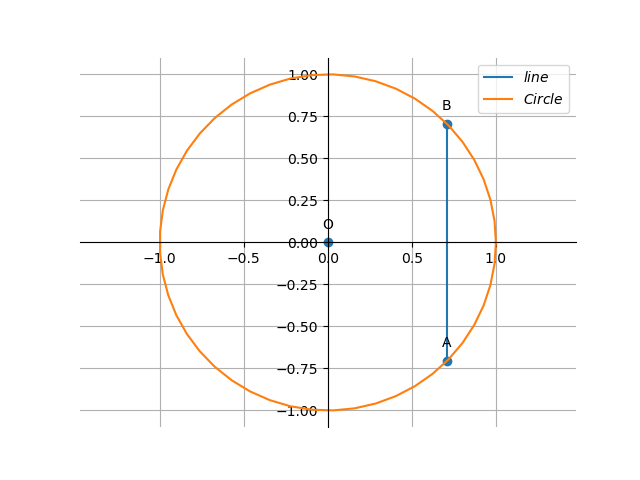
\includegraphics[width=\columnwidth]{chapters/12/8/1/7/figs/conic.png}
		\caption{}
		\label{fig:12/8/1/7}
  	\end{figure}
The given circle can be expressed as a conic with parameters
\begin{align}
\vec{V}=
\myvec{
1 & 0\\
0 & 1
},
\vec{u}=0,
f=-a^2
\end{align} 
The given line 
parameters are
\begin{align} 
	\vec{h}=\myvec{\frac{a}{\sqrt{2}} \\ 0},  \vec{m}=\vec{e}_2.
\end{align}
Substituting the above in
\eqref{eq:tangent_roots},
\begin{align}
    \kappa =\pm\frac{a}{\sqrt{2}}
\end{align}
yielding the
points of intersection of the line with circle as
\begin{align}
    \vec{A}=\myvec{
\frac{a}{\sqrt{2}}\\
-\frac{a}{\sqrt{2}}
    },
    \vec{B}=\myvec{
\frac{a}{\sqrt{2}}\\
\frac{a}{\sqrt{2}}
    }
\end{align}
 From 
		\figref{fig:12/8/1/7},
the total area of the portion is given by
\begin{align}
	ar( APQ)&=2 ar (APR)
	\\
&=2\int_{0}^{\frac{a}{\sqrt{2}}}\sqrt{a^2-x^2}\,dx 
	\\
	&=\frac{a^2}{2}\brak{1+\frac{\pi}{2}}
\end{align}
